\section{Connection}

\subsection{Connection message system}

Beskeder i systemet foregår via en række objekter, der alle nedarver fra en basis klasse ved navn Message. Disse er beskrevet nærmere i følgende afsnit

\subsubsection{Message}
Indeholder en enum af typen MessageTypes, hvori alle typer beskeder fremgår. Desuden indeholder den en string med MessageInfo, som primært anvendes i tilfælde af fejl, hvor beskeden vises i systemets GUI som vist på figur~\ref{fig:loginError}

\begin{figure}
	\centering
	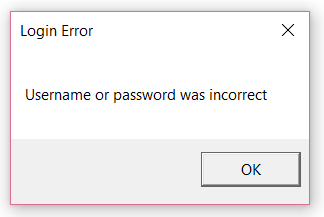
\includegraphics[width=0.5\linewidth]{figs/connection/loginError.png}
	\caption{WinLoginView}
	\label{fig:loginError}
\end{figure}

Nedarving fra message klassen er vist på figur~\ref{fig:MessageUML}

\begin{figure}
	\centering
	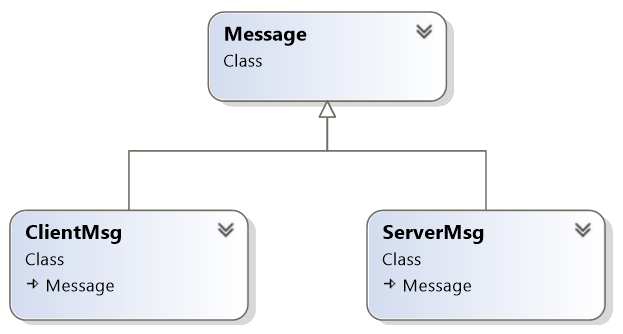
\includegraphics[width=0.7\linewidth]{figs/connection/MessageUML.png}
	\caption{WinLoginView}
	\label{fig:MessageUML}
\end{figure}

\subsubsection{ClientMsg}
Indeholder ikke yderligere informationer, men definerer en adskillelse mellem server beskeder og klient beskeder. Desuden giver det mulighed for at alle klient beskeder i fremtiden kan indeholder informationer, som server beskeder ikke indeholder. Nedarving fra ClientMsg klassen er vist på figur~\ref{fig:ClientMsgUML}

\begin{figure}
	\centering
	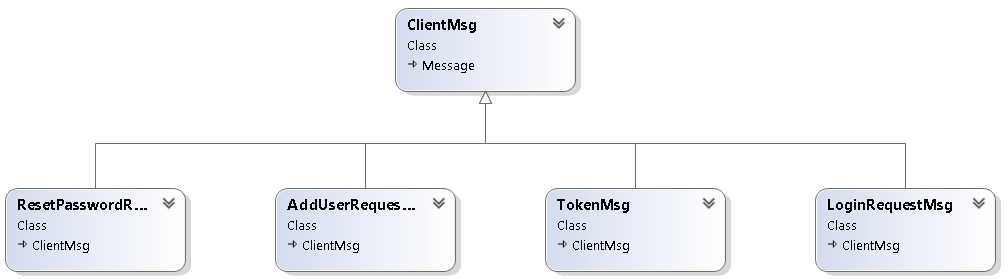
\includegraphics[width=0.9\linewidth]{figs/connection/ClientMsgUML.png}
	\caption{WinLoginView}
	\label{fig:ClientMsgUML}
\end{figure}

\paragraph{ResetPasswordRequestMsg}
\begin{lstlisting}[caption=ResetPasswordRequestMsg, label=code:ResetPasswordRequestMsg]
public class ResetPasswordRequestMsg : ClientMsg
{
	public string Username { get; set; }
	
	public ResetPasswordRequestMsg(string username)
	{
		Username = username;
		MsgType = MessageTypes.ResetPasswordRequest;
	}
}
\end{lstlisting}

\paragraph{AddUserRequestMsg}
Indeholder de informationer der bliver gemt i databasen når en bruger bliver oprettet.
\begin{lstlisting}[caption=AddUserRequestMsg, label=code:AddUserRequestMsg]
public class AddUserRequestMsg : ClientMsg
{
	public string Fullname { get; set; }
	public string Username { get; set; }
	public string Password { get; set; }
	
	public AddUserRequestMsg(string fullname, string username, string password)
	{
		Fullname = fullname;
		Username = username;
		Password = password;
		MsgType = MessageTypes.AddUserRequest;
	}
}
\end{lstlisting}

\paragraph{LoginRequestMsg}
\begin{lstlisting}[caption=LoginRequestMsg, label=code:LoginRequestMsg]
public class LoginRequestMsg : ClientMsg
{
	public string Username { get; set; }
	public string Password { get; set; }
	
	public LoginRequestMsg(string username, string password)
	{
		Username = username;
		Password = password;
		MsgType = MessageTypes.LoginRequest;
	}
}
\end{lstlisting}

\subsubsection{TokenMsg}
\begin{lstlisting}[caption=TokenMsg, label=code:TokenMsg]
public class TokenMsg : ClientMsg
{
	public string Username { get; set; }
	public string TokenString { get; set; }
	public TokenSubMessageTypes SubMsgType { get; set; }
	
	public TokenMsg(string username, string tokenString)
	{
		Username = username;
		TokenString = tokenString;
		MsgType = MessageTypes.TokenMsg;
	}
}
\end{lstlisting}

Nedarving fra TokenMsg er vist på figur~\ref{fig:TokenMsgUML}. AddPoolPictureRequestMsg er ikke blevet implementeret 
\begin{figure}
	\centering
	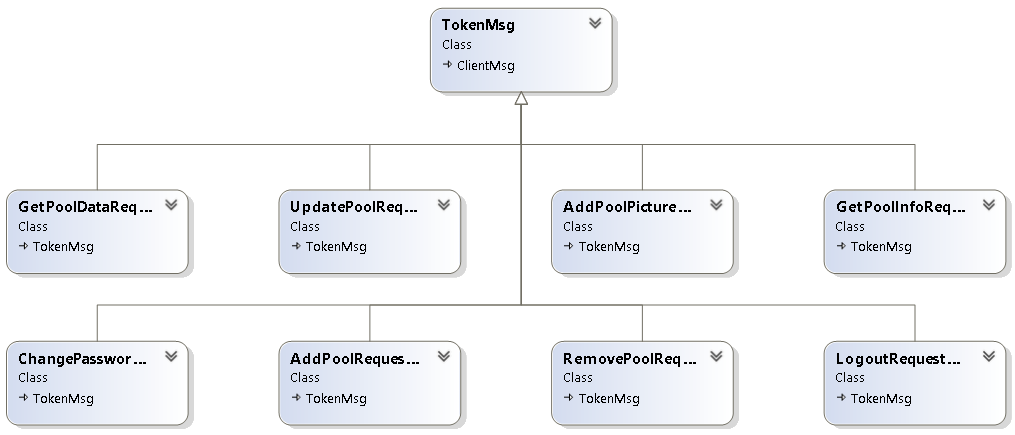
\includegraphics[width=0.7\linewidth]{figs/connection/TokenMsgUML.png}
	\caption{WinLoginView}
	\label{fig:TokenMsgUML}
\end{figure}

\paragraph{AddPoolRequest}
\begin{lstlisting}[caption=AddPoolRequest, label=code:AddPoolRequest]
public class AddPoolRequestMsg : TokenMsg
{
	public string PoolName { get; set; }
	public double Volume { get; set; }
	public string SerialNumber { get; set; }
	
	public AddPoolRequestMsg(string username, string tokenString, string poolName, double poolVolume, string serialNumber) : base(username, tokenString)
	{
		PoolName = poolName;
		Volume = poolVolume;
		SerialNumber = serialNumber;
		SubMsgType = TokenSubMessageTypes.AddPoolRequest;
	}
}
\end{lstlisting}

\paragraph{GetPoolDataRequest}
\begin{lstlisting}[caption=GetPoolDataRequest, label=code:GetPoolDataRequest]
public class GetPoolDataRequestMsg : TokenMsg
{
	public bool GetAllNamesOnly { get; set; }
	public string PoolName { get; set; }
	public int GetHistoryDays { get; set; }
	
	public GetPoolDataRequestMsg(string username, string tokenString, bool getAllNamesOnly = false, string poolName = "", int getHistoryDays = 0)
	: base(username, tokenString)
	{
		GetAllNamesOnly = getAllNamesOnly;
		PoolName = poolName;
		GetHistoryDays = getHistoryDays;
		SubMsgType = TokenSubMessageTypes.GetPoolDataRequest;
	}
}
\end{lstlisting}

\paragraph{GetPoolInfoRequest}
\begin{lstlisting}[caption=GetPoolInfoRequest, label=code:GetPoolInfoRequest]
public class GetPoolInfoRequestMsg : TokenMsg
{
	public string PoolName { get; set; }
	
	public GetPoolInfoRequestMsg(string username, string tokenString, string poolName) : base(username, tokenString)
	{
		PoolName = poolName;
		SubMsgType = TokenSubMessageTypes.GetPoolInfoRequest;
	}
}
\end{lstlisting}

\paragraph{RemovePoolRequest}
\begin{lstlisting}[caption=RemovePoolRequest, label=code:RemovePoolRequest]
public class RemovePoolRequestMsg : TokenMsg
{
	public string PoolName { get; set; }
	
	public RemovePoolRequestMsg(string username, string tokenString, string poolName) : base(username, tokenString)
	{
		PoolName = poolName;
		SubMsgType = TokenSubMessageTypes.RemovePoolRequest;
	}
}
\end{lstlisting}

\paragraph{UpdatePoolRequest}
\begin{lstlisting}[caption=UpdatePoolRequest, label=code:UpdatePoolRequest]
public class UpdatePoolRequestMsg : TokenMsg
{
	public string OldPoolName { get; set; }
	public string NewPoolName { get; set; }
	public double NewPoolVolume { get; set; }
	
	public UpdatePoolRequestMsg(string username, string tokenString, string oldPoolName, string newPoolName = "", double newPoolVolume = 0) : base(username, tokenString)
	{
		OldPoolName = oldPoolName;
		NewPoolName = newPoolName;
		NewPoolVolume = newPoolVolume;
		SubMsgType = TokenSubMessageTypes.UpdatePoolRequest;
	}
}
\end{lstlisting}

\paragraph{ChangePasswordRequest}
\begin{lstlisting}[caption=ChangePasswordRequest, label=code:ChangePasswordRequest]
public class ChangePasswordRequestMsg : TokenMsg
{
	public string OldPassword { get; set; }
	public string NewPassword { get; set; }
	
	public ChangePasswordRequestMsg(string username, string tokenString, string oldPassword, string newPassword) : base(username, tokenString)
	{
		OldPassword = oldPassword;
		NewPassword = newPassword;
		SubMsgType = TokenSubMessageTypes.ChangePasswordRequest;
	}
}
\end{lstlisting}

\paragraph{LogoutRequest}
\begin{lstlisting}[caption=LogoutRequest, label=code:LogoutRequest]
public class LogoutRequestMsg : TokenMsg
{
	public LogoutRequestMsg(string username, string tokenString) : base(username, tokenString)
	{
		SubMsgType = TokenSubMessageTypes.LogoutRequest;
	}
}
\end{lstlisting}

\subsubsection{ServerMsg}
Nedarving fra ServerMsg er vist på figur~\ref{fig:ServerMsgUML}
\begin{figure}
	\centering
	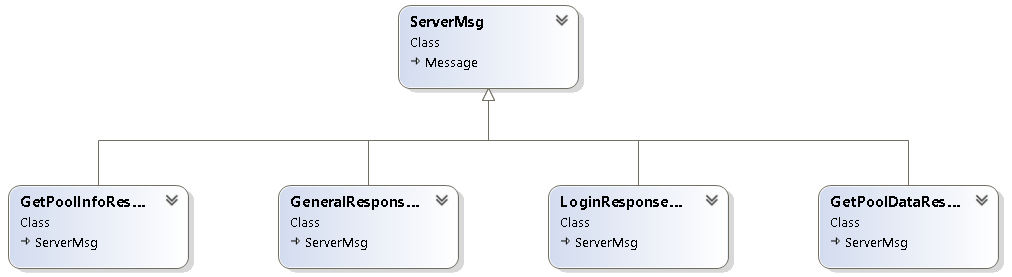
\includegraphics[width=0.7\linewidth]{figs/connection/ServerMsgUML.png}
	\caption{WinLoginView}
	\label{fig:ServerMsgUML}
\end{figure}

\paragraph{GeneralResponseMsg}
\begin{lstlisting}[caption=GeneralResponseMsg, label=code:GeneralResponseMsg]
public class GeneralResponseMsg : ServerMsg
{
	public bool TokenStillActive { get; set; }
	public bool RequestExecutedSuccesfully { get; set; }
	public GeneralResponseMsg(bool tokenStillActive, bool requestExecutedSuccesfully)
	{
		TokenStillActive = tokenStillActive;
		RequestExecutedSuccesfully = requestExecutedSuccesfully;
		MsgType = MessageTypes.GeneralResponse;
	}
}
\end{lstlisting}

\paragraph{GetPoolDataResponse}
\begin{lstlisting}[caption=GetPoolDataResponse, label=code:GetPoolDataResponse]
public class GetPoolDataResponseMsg : ServerMsg
{
	public List<Tuple<SensorTypes, List<double>>> SensorList { get; set; }
	public List<Tuple<string, bool>> AllPoolNamesListTuple { get; set; }
	
	public GetPoolDataResponseMsg(List<Tuple<SensorTypes, List<double>>> sensorList = null, List<Tuple<string, bool>> allPoolNamesListTuple = null )
	{
		SensorList = sensorList;
		AllPoolNamesListTuple = allPoolNamesListTuple;
		MsgType = MessageTypes.GetPoolDataResponse;
	}
}
\end{lstlisting}

\paragraph{GetPoolInfoResponse}
\begin{lstlisting}[caption=GetPoolInfoResponse, label=code:GetPoolInfoResponse]
public class GetPoolInfoResponseMsg : ServerMsg
{
	public double Volume { get; set; }
	public string SerialNumber { get; set; }
	
	public GetPoolInfoResponseMsg(double volume, string serialNumber)
	{
		Volume = volume;
		SerialNumber = serialNumber;
		MsgType = MessageTypes.GetPoolInfoResponse;
	}
}
\end{lstlisting}

\paragraph{LoginResponse}
\begin{lstlisting}[caption=LoginResponse, label=code:LoginResponse]
public class LoginResponseMsg : ServerMsg
{
	public string TokenString { get; set; }
	public bool LoginSuccessful { get; set; }
	
	public LoginResponseMsg(string tokenString, bool loginSuccessful)
	{
		TokenString = tokenString;
		LoginSuccessful = loginSuccessful;
		MsgType = MessageTypes.LoginResponse;
	}
}
\end{lstlisting}

\subsection{Client}

\subsubsection{Synchronous Socket Client}

\subsubsection{ClientMessenger}

\subsubsection{Client Response Manager}

\subsection{Server}

\subsubsection{Asynchronous Socket Listener}
Den primære funktionalitet af denne klasse er hentet fra https://msdn.microsoft.com/en-us/library/fx6588te(v=vs.110).aspx ?? . Denne fungerer ved at køre asynchront, hvilket vil sige at applikationen ikke idler når der afventes en connection. Dette vil med andre ord sige, at der kan oprettes flere forbindelser til serveren på samme tid, da de ikke blokkerer hinanden.
Der er ændret i klassens konsol output, så essentielle data vises. Dette kan ses på figur~\ref{fig:asynchronousSocketListener}

\begin{figure}
	\centering
	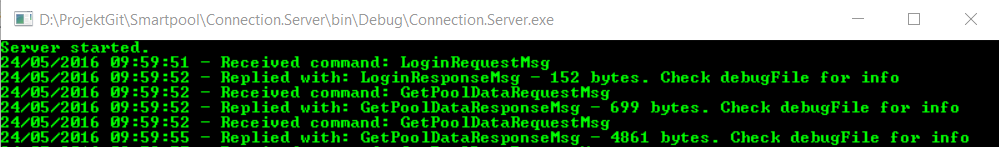
\includegraphics[width=0.9\linewidth]{figs/connection/asynchronousSocketListener.png}
	\caption{WinLoginView}
	\label{fig:asynchronousSocketListener}
\end{figure}

Udfra de viste informationer kan man hurtigt se hvilken type besked der er modtaget, samt hvilken type besked der er svaret med, samt hvor meget denne besked fylder. Det fulde output bliver desuden gemt i en log fil, så det efterfølgende er muligt at se præcis hvilke informationer der er sendt. Dette er valgt for at gøre server vinduet overskueligt, uden at miste essentielle informationer.

Der er desuden valgt at lade exceptions blive vist i server vinduet, som f.eks. ses på figur~\ref{fig:asynchronousSocketListenerException} hvor databasen har genereret en exception, da der er forsøgt at lave et login med et ukendt brugernavn.

\begin{figure}
	\centering
	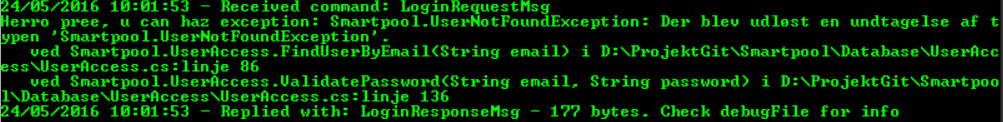
\includegraphics[width=0.9\linewidth]{figs/connection/asynchronousSocketListenerException.png}
	\caption{WinLoginView}
	\label{fig:asynchronousSocketListenerException}
\end{figure}

Som det også fremgår i server vinduet figur~\ref{fig:asynchronousSocketListenerException} bliver en exception håndteret af serveren, og der sendes en besked af den korrekte type tilbage til klient applikationen, så hverken server eller klient crasher.

\subsubsection{Response Manager}

\subsubsection{Token System}

\subsubsection{FakePool DataGeneration}

